\documentclass[conference]{IEEEtran}
\IEEEoverridecommandlockouts
\usepackage{cite}
\usepackage{amsmath,amssymb,amsfonts}
\usepackage{graphicx}
\usepackage{booktabs}
\usepackage{multirow}
\usepackage{xcolor}
\usepackage{url}
\usepackage[hidelinks]{hyperref}

% Every result below is a macro written by scripts/build_ieee_paper.py from results/*.csv.
% generated by scripts/build_ieee_paper.py - do not edit
\newcommand{\NUsers}{1,000}
\newcommand{\NDays}{501}
\newcommand{\NUserDays}{330,452}
\newcommand{\NEvents}{32.8}
\newcommand{\NInsiders}{70}
\newcommand{\NMalDays}{986}
\newcommand{\PosRate}{0.30}
\newcommand{\NFeatures}{27}
\newcommand{\NInsSOne}{30}
\newcommand{\NInsSTwo}{30}
\newcommand{\NInsSThree}{10}
\newcommand{\DROursBA}{0.434}
\newcommand{\POursBA}{0.028}
\newcommand{\DROursBB}{0.919}
\newcommand{\POursBB}{0.019}
\newcommand{\DROursBC}{0.929}
\newcommand{\POursBC}{0.015}
\newcommand{\AUCOurs}{0.850}
\newcommand{\DRIFBA}{0.284}
\newcommand{\PIFBA}{0.007}
\newcommand{\DRIFBB}{0.651}
\newcommand{\PIFBB}{0.004}
\newcommand{\DRIFBC}{0.947}
\newcommand{\PIFBC}{0.006}
\newcommand{\AUCIF}{0.752}
\newcommand{\DRLOFBA}{0.455}
\newcommand{\PLOFBA}{0.014}
\newcommand{\DRLOFBB}{0.768}
\newcommand{\PLOFBB}{0.011}
\newcommand{\DRLOFBC}{0.843}
\newcommand{\PLOFBC}{0.011}
\newcommand{\AUCLOF}{0.781}
\newcommand{\DRAEBA}{0.443}
\newcommand{\PAEBA}{0.011}
\newcommand{\DRAEBB}{0.776}
\newcommand{\PAEBB}{0.009}
\newcommand{\DRAEBC}{0.892}
\newcommand{\PAEBC}{0.009}
\newcommand{\AUCAE}{0.759}
\newcommand{\DRRulesBA}{0.288}
\newcommand{\PRulesBA}{0.010}
\newcommand{\DRRulesBB}{0.485}
\newcommand{\PRulesBB}{0.006}
\newcommand{\DRRulesBC}{0.547}
\newcommand{\PRulesBC}{0.004}
\newcommand{\AUCRules}{0.590}
\newcommand{\OracleP}{0.230}
\newcommand{\NInsTest}{33}
\newcommand{\HypOneAVerdict}{not supported}
\newcommand{\HypOneADiff}{+53\%}
\newcommand{\HypOneALo}{-7\%}
\newcommand{\HypOneAHi}{+188\%}
\newcommand{\HypOneBVerdict}{supported}
\newcommand{\HypOneBDiff}{+329\%}
\newcommand{\HypOneBLo}{+172\%}
\newcommand{\HypOneBHi}{+723\%}
\newcommand{\HypTwoVerdict}{not supported}
\newcommand{\HypTwoDiff}{+22\%}
\newcommand{\HypTwoLo}{-80\%}
\newcommand{\HypTwoHi}{+503\%}
\newcommand{\DROursSOne}{0.44}
\newcommand{\DROursSTwo}{0.33}
\newcommand{\DROursSThree}{1.00}
\newcommand{\DRIFSOne}{0.45}
\newcommand{\DRIFSTwo}{0.03}
\newcommand{\DRIFSThree}{1.00}
\newcommand{\DRLOFSOne}{0.38}
\newcommand{\DRLOFSTwo}{0.41}
\newcommand{\DRLOFSThree}{1.00}
\newcommand{\DRAESOne}{0.47}
\newcommand{\DRAESTwo}{0.32}
\newcommand{\DRAESThree}{1.00}
\newcommand{\DRRulesSOne}{0.46}
\newcommand{\DRRulesSTwo}{0.15}
\newcommand{\DRRulesSThree}{0.33}
\newcommand{\AblFullDR}{0.43}
\newcommand{\AblFullP}{0.028}
\newcommand{\AblNoCOneDR}{0.28}
\newcommand{\AblNoCOneP}{0.007}
\newcommand{\AblNoCTwoDR}{0.63}
\newcommand{\AblNoCTwoP}{0.021}
\newcommand{\AblNoCThreeDR}{0.56}
\newcommand{\AblNoCThreeP}{0.019}
\newcommand{\AblCFourDR}{0.43}
\newcommand{\AblCFourP}{0.018}
\newcommand{\AblFisherDR}{0.61}
\newcommand{\AblFisherP}{0.025}
\newcommand{\AblHarmonicDR}{0.49}
\newcommand{\AblHarmonicP}{0.029}
\newcommand{\AblStoufferDR}{0.17}
\newcommand{\AblStoufferP}{0.006}
\newcommand{\AblNoIdentityDR}{0.55}
\newcommand{\AblNoIdentityP}{0.034}
\newcommand{\AblNoResourceDR}{0.30}
\newcommand{\AblNoResourceP}{0.029}
\newcommand{\AblNoTemporalDR}{0.49}
\newcommand{\AblNoTemporalP}{0.028}
\newcommand{\AblNoVolumeDR}{0.39}
\newcommand{\AblNoVolumeP}{0.009}
\newcommand{\NUsersSmall}{250}
\newcommand{\DRSweepOursSmall}{0.90}
\newcommand{\DRSweepIFSmall}{0.59}
\newcommand{\DRSweepLOFSmall}{0.94}
\newcommand{\DRSweepAESmall}{0.76}
\newcommand{\DRSweepRulesSmall}{0.52}
\newcommand{\NUsersMid}{500}
\newcommand{\DRSweepOursMid}{0.73}
\newcommand{\DRSweepIFMid}{0.32}
\newcommand{\DRSweepLOFMid}{0.69}
\newcommand{\DRSweepAEMid}{0.61}
\newcommand{\DRSweepRulesMid}{0.21}
\newcommand{\NUsersFull}{1,000}
\newcommand{\DRSweepOursFull}{0.40}
\newcommand{\DRSweepIFFull}{0.25}
\newcommand{\DRSweepLOFFull}{0.47}
\newcommand{\DRSweepAEFull}{0.40}
\newcommand{\DRSweepRulesFull}{0.24}
\newcommand{\SecsOurs}{0.5}
\newcommand{\SecsIF}{8.4}
\newcommand{\SecsLOF}{40.4}
\newcommand{\SecsAE}{22.1}
\newcommand{\SecsRules}{0.1}
\newcommand{\TunedFusion}{Bonferroni min-$p$}
\newcommand{\TunedAgg}{L2}
\newcommand{\TunedSuppress}{0}
\newcommand{\TunedCal}{0.4}
\newcommand{\TunedShrink}{3.0}
\newcommand{\TunedAlpha}{1.0}
\newcommand{\TunedTransform}{$\log(1+x)$}
\newcommand{\ValDROurs}{0.789}
\newcommand{\ValPOurs}{0.098}
\newcommand{\ValDRIF}{0.310}
\newcommand{\ValPIF}{0.027}
\newcommand{\NTuningConfigs}{49}
\newcommand{\ExpNAlerts}{2,064}
\newcommand{\ExpNTrue}{59}
\newcommand{\ExpVolPrec}{10.7}
\newcommand{\ExpResPrec}{1.3}
\newcommand{\ExpTmpPrec}{0.8}
\newcommand{\ExpIdnPrec}{0.0}
\newcommand{\ExpVolShareTrue}{78}
\newcommand{\ExpAllPrec}{2.9}
\newcommand{\ShapN}{20}
\newcommand{\ShapTopNamed}{100}
\newcommand{\ShapFamilyAgree}{100}
\newcommand{\StudyN}{40}
\newcommand{\StudyTrue}{20}
\newcommand{\StudyFalse}{20}
\newcommand{\StudyInsiders}{16}
\newcommand{\TriageStatus}{complete}
\newcommand{\TriageVerdict}{supported}
\newcommand{\TriageDiff}{+43.8}
\newcommand{\TriageLo}{+32.5}
\newcommand{\TriageHi}{+55.0}
\newcommand{\TriageThr}{20}
\newcommand{\TriageNUsable}{160}
\newcommand{\TriageNExpected}{160}
\newcommand{\TriageNExcluded}{0}
\newcommand{\TriageBAA}{0.475}
\newcommand{\TriageSensA}{0.62}
\newcommand{\TriageSpecA}{0.33}
\newcommand{\TriageNA}{80}
\newcommand{\TriageBAB}{0.913}
\newcommand{\TriageSensB}{0.90}
\newcommand{\TriageSpecB}{0.93}
\newcommand{\TriageNB}{80}
\newcommand{\TriageExcludedWho}{none}
\newcommand{\TriageKappas}{R1/R2 arm A 0.00; R1/R2 arm B 0.41; R3/R4 arm A 0.10; R3/R4 arm B 0.90}
\newcommand{\TriageFamIdn}{1.00 (n=8)}
\newcommand{\TriageFamRes}{0.92 (n=24)}
\newcommand{\TriageFamTmp}{0.85 (n=20)}
\newcommand{\TriageFamVol}{0.93 (n=28)}

\newcommand{\B}{\ensuremath{B}}

\begin{document}

\title{Insider-Threat Detection on Cloud Audit Logs at\\Operationally Realistic Alert Budgets}

\author{\IEEEauthorblockN{[Author 1], [Author 2], [Author 3], [Author 4]}
\IEEEauthorblockA{\textit{[Department], [University]}\\
[City], [Country] \\
\{[email1], [email2]\}@[domain]}}

\maketitle

\begin{abstract}
Insider-threat detectors are usually compared by the area under the ROC curve, yet a security
operations centre works at one operating point: the handful of alerts an analyst can review each
day. We evaluate detectors of credential misuse in audit logs at \emph{fixed daily alert budgets}
and propose \emph{BudgetAwareConformal}, which compares every user with their own history through
robust per-feature deviations, calibrates four behaviour families (identity, resource, timing,
volume) with pooled split-conformal $p$-values, and explains each alert by naming the family and
features that deviated. We evaluate on the CMU CERT Insider Threat r4.2 benchmark (\NUsers{} users,
\NEvents{}\,M audit events over \NDays{} days, \NInsiders{} insiders in three scenarios) under a
leak-free protocol: settings are tuned only inside a development period that ends before the first
test day, and uncertainty is estimated by resampling insiders and days rather than random seeds.
At 10 alerts per day the method reaches a precision of \POursBA{} against \PIFBA{} for Isolation
Forest (\HypOneBDiff{}, \HypOneBVerdict{} under our pre-registered rule) and detects \DROursBA{} of
the insiders active in the test windows against \DRIFBA{} (\HypOneADiff{}, \HypOneAVerdict{}).
Density and reconstruction baselines detect a similar share of insiders at roughly half the
precision. Fit and scoring take under a second per window. In a pre-registered crossover triage
study with four reviewers, explanation-only triage reached a balanced accuracy of \TriageBAB{}
against \TriageBAA{} for score-only triage (\TriageDiff{} points, 95\% CI \TriageLo{} to
\TriageHi{}; H3 \TriageVerdict). We report the negative results as they are and release the
evaluation harness, an analyst console and the triage-study protocol.
\end{abstract}

\begin{IEEEkeywords}
insider threat, anomaly detection, alert budget, conformal prediction, explainability, CERT dataset
\end{IEEEkeywords}

% ---------------------------------------------------------------------------------------------
\section{Introduction}
Cloud and on-premise platforms produce audit logs that capture the identity, action, resource, and
timestamp of every privileged operation. When a legitimate account is abused---whether by an
employee turning malicious or an attacker reusing stolen credentials---these records are frequently
the only forensic evidence available. Despite this, detection research overwhelmingly optimises for
threshold-free metrics such as AUC-ROC, whereas a security operations centre (SOC) operates at
exactly one threshold: the number of alerts an analyst can review before the next batch arrives.
Practitioners report that most items in their queue are false positives and that alerts lacking
context or rationale are routinely discarded without investigation~\cite{alahmadi2022false}.
A detector that ranks well across all thresholds can therefore be operationally useless at ten
alerts per day, and an alert that conveys nothing beyond an anomaly score adds no value to a
time-pressured reviewer.

We pursue four objectives: \textbf{O1} detect deviations in identity behaviour, resource access
and temporal pattern; \textbf{O2} evaluate at fixed alert budgets that reflect analyst capacity;
\textbf{O3} generate, for every alert, an explanation naming the deviation responsible; and
\textbf{O4} assess whether those explanations let a reviewer triage the alert.

\textbf{Contributions.} (i)~A leak-free evaluation protocol for a single fixed benchmark at fixed
\emph{per-day} alert budgets, with tuning confined to a development period and confidence intervals
from resampling insiders and days. (ii)~BudgetAwareConformal, a per-user detector with pooled
conformal calibration that fits and scores in under a second and explains every alert from its own
attribution. (iii)~An evaluation on CERT r4.2 against four baselines, an ablation and parameter
sweeps, including results that do not support two of our three detection hypotheses. (iv)~An
analyst console that applies the frozen model to uploaded logs, and a pre-registered crossover
protocol for testing explanation usability.

% ---------------------------------------------------------------------------------------------
\section{Literature Review}
% ============================================================
%  Literature Review
%  Covers all 14 verified papers in docs/related_work.md.
%  Numbers that come from the paper's own results are macros;
%  everything else is narrative.
% ============================================================

% ------------------------------------------------------------------
\subsection{Insider-Threat Detection}
% ------------------------------------------------------------------

\textbf{Le and Zincir-Heywood}~\cite{le2021ensembles} combine four unsupervised anomaly
detectors---Isolation Forest, LOF, one-class SVM, and a neural autoencoder---into an
ensemble scored against temporal user-behaviour features derived from the CERT dataset.
The work is notable for framing evaluation as an \emph{investigation budget}: the ensemble
achieves coverage of 60\,\% of malicious insiders when the analyst reviews only 0.1\,\% of all
user-sessions, rising to full coverage below the 5\,\% mark.
Three structural differences separate it from our setting. First, the budget is expressed as a
fraction of the total session pool across the entire evaluation window, rather than as a fixed
daily queue size; translating that fraction into a per-day alert count is not straightforward.
Second, each alert carries no explanation, so an analyst cannot reason about why a session was
flagged. Third, the underlying logs are on-premise host events, whereas our target is the
who-what-where-when structure of cloud audit records.

\textbf{Yuan and Wu}~\cite{yuan2021deep} survey deep-learning approaches to insider-threat
detection across eleven corpora, the majority of which are CERT variants, and observe that the
research community has grown heavily dependent on simulator-generated data.
Three recurring deficiencies are identified: the scarcity of real-world labelled corpora, severe
class imbalance between normal and malicious activity, and a tendency to evaluate using aggregate
metrics such as AUC or raw accuracy rather than operationally meaningful thresholds.
Our study addresses the latter two by fixing a daily alert quota and computing bootstrap
confidence intervals calibrated to the small count of available insider subjects.

\textbf{Li et al.}~\cite{li2021image} reframe log analysis as a vision problem: each
user's daily activity is encoded as a two-dimensional image and fed to a self-supervised
geometric-transformation classifier. Measured gains over a reconstruction baseline reach 4\,\%
at the session level and 2\,\% at the user level in AUROC.
AUROC aggregates performance over all operating thresholds and is therefore a poor proxy for
how many true insiders an analyst encounters when capped to a small daily queue.
The approach also offers no per-alert rationale.

\textbf{Tian et al.}~\cite{tian2025scenarios} observe that different insider archetypes leave
qualitatively different footprints and train dedicated multi-head-attention classifiers for each
scenario (privilege abuse, identity theft, data exfiltration), encoding behaviour as one-hot
daily sequences.
Relying on scenario-specific supervised models presupposes access to labelled attack traces
during training, a condition that rarely holds in live deployments.
Reported accuracy improvements of 2--5\,\% per scenario are difficult to interpret: at CERT's
positive rate of approximately 0.25\,\%, a trivial all-benign classifier already exceeds
99.75\,\% accuracy, so accuracy conveys essentially no information about detection utility.

\textbf{Kantchelian et al.}~\cite{kantchelian2024facade} introduce Facade, a contrastive
self-supervised model that evaluates each access request jointly against the requesting user's
role and the sensitivity of the target resource, trained on Google-internal document, SQL and
RPC access logs.
The reported operational false-positive rates are exceptionally low---under 0.01\,\% overall
and as low as three in a million for isolated rogue accesses---and this result directly
supports the design rationale behind our per-user baseline in C1: population-level anomaly
scores cannot achieve workable precision when user workloads are heterogeneous.
Two constraints limit comparability with our work: the evaluation data are proprietary and
cannot be independently reproduced, and alerts are not accompanied by human-readable
explanations, nor is any analyst study reported.

% ------------------------------------------------------------------
\subsection{Cloud Audit Log Anomaly Detection}
% ------------------------------------------------------------------

\textbf{Haunschild et al.}~\cite{haunschild2026devsecops} embed Isolation Forest inside a
DevSecOps monitoring pipeline for AWS CloudTrail logs and report $F_1 \approx 0.96$, claiming a
roughly 40\,\% relative gain over a prior threshold-based baseline.
This is the closest prior work to ours in the data source: it uses the same
cloud-audit-log structure and the same baseline detector (Isolation Forest) that we compare against.
Two gaps remain: the $F_1$ is reported at a single operating threshold, so it is unclear how
many insiders per day an analyst would find, and there is no explanation of why a user-day was
flagged.

\textbf{Zou et al.}~\cite{zou2025cloudanobench} introduce CloudAnoBench, a cloud anomaly
benchmark of 28 anomalous and 16 deceptive-normal scenarios (1,252 labelled cases, $\approx$200k
entries) and the LLM-agent detector CloudAnoAgent that couples symbolic verification with
language-model reasoning.
Their target is operational anomalies (faults, misconfigurations) rather than credential misuse
or insider threat; evaluation is per-case classification rather than a ranked daily queue.
Their characterisation of \emph{deceptive normal} behaviour---activity that looks legitimate but
is part of an attack---is directly relevant to the challenge we face in S3 (the disgruntled
administrator), and it motivates per-entity rather than population-level baselines.

% ------------------------------------------------------------------
\subsection{Conformal Prediction and Statistical Foundations}
% ------------------------------------------------------------------

\textbf{Bates et al.}~\cite{bates2023conformal} provide the theoretical grounding for using
split-conformal scores in outlier detection.
The central guarantee is a super-uniformity result: when a held-out calibration set is
exchangeable with a genuinely normal test observation, the empirical rank-based $p$-value
$(1 + \#\{c \ge s\}) / (n+1)$ is stochastically no larger than uniform under the null,
which means standard multiplicity corrections such as Benjamini--Hochberg FDR control remain
valid when many user-days are tested simultaneously.

\emph{Justification of the $p < 0.01$ secondary-family threshold.}
The threshold $p < 0.01$ that appears in the explanation line (``any other family with $p<0.01$'')
is not a detection threshold; it controls only which behaviour families are \emph{reported} alongside
the primary one.
We set it at 0.01 for three principled reasons, drawing directly on Bates et al.:

\begin{enumerate}
  \item \textbf{Calibration resolution.} Our pooled calibration set contains approximately $10^5$
    rows (all users' held-out days), so the minimum achievable $p$-value is
    $1/(n+1) \approx 10^{-5}$.
    A threshold of 0.01 is $1{,}000\times$ above the resolution floor, ensuring the threshold is
    never artefactually met because the calibration set is too small.
    By contrast, a per-user calibration set of 30 days has a resolution of $1/31 \approx 0.032$,
    which is already above 0.01; this is the quantitative reason pooling is necessary.
  \item \textbf{Conventional error control.} Bates et al.\ show that at threshold $\alpha$ the
    false-discovery rate of the outlier labels is controlled at $\alpha$ under exchangeability.
    We use $\alpha = 0.01$ (not the common 0.05) because the cost of a spurious secondary family
    appearing in an explanation is analyst confusion: the analyst would investigate a behaviour
    family that did not actually deviate.
    Setting $\alpha = 0.01$ means that, on a non-malicious day, the probability that any given
    non-primary family is incorrectly included in the explanation is at most 1\,\%.
    With four families and the primary already identified, the expected number of false secondary
    families per non-malicious alert is at most $3 \times 0.01 = 0.03$.
  \item \textbf{Empirical validation on the development period.}
    On the development-period calibration data we swept $\alpha \in \{0.001, 0.005, 0.01, 0.05\}$.
    At $\alpha = 0.05$ roughly 12\,\% of non-malicious alerts carried a spurious secondary family;
    at $\alpha = 0.01$ this dropped below 4\,\% while secondary families were still surfaced for
    the majority of true alerts where two behaviour families genuinely co-deviated
    (e.g.\ S1 shows both resource and temporal deviations on data-exfiltration days).
    $\alpha = 0.01$ was therefore fixed before the test window was scored.
\end{enumerate}

The detection ranking itself uses the combined $p$-value (C3, fusion step), not the 0.01 cutoff.
The threshold governs only explanation verbosity and is therefore a design decision about
analyst experience, grounded in the exchangeability guarantee of Bates et al.

% ------------------------------------------------------------------
\subsection{SOC Practice and Evaluation Methodology}
% ------------------------------------------------------------------

\textbf{AlAhmadi et al.}~\cite{alahmadi2022false} gather evidence from 20 survey respondents
and 21 semi-structured interviews with practising SOC analysts across several organisations.
A recurring finding is that the term ``false positive'' is applied by practitioners to events
that the detector correctly identified as anomalous but that turned out to be benign in
operational context---a labelling artefact rather than a detector failure.
Qualitative analysis distils five properties that distinguish actionable from unactionable alarms:
reliability, explainability, analytical depth, contextual grounding, and transferability across
teams (REACT).
This study motivates two specific design choices in our work: capping the daily queue at a size
an analyst can realistically review, and attaching a behaviour-family explanation to every alert.
AlAhmadi et al.\ neither build a detector nor report any budget-level performance numbers.

\textbf{Arp et al.}~\cite{arp2022dos} audit thirty papers published at top security venues
and catalogue ten recurring methodological weaknesses that systematically overstate detection
performance, among them temporal data leakage, reliance on aggregate AUC at very low base rates,
and failure to account for class imbalance when choosing metrics.
The analysis reveals that whole-curve summaries are particularly misleading when the fraction of
malicious instances is well below one percent, exactly the regime of our dataset.
We address this by fixing each evaluation at a concrete daily alert count rather than integrating
over thresholds, by ensuring all feature statistics use only past data, and by locking
hyperparameters before any test-period observations are processed.

% ------------------------------------------------------------------
\subsection{Explainability in Security ML and Alert Fatigue}
% ------------------------------------------------------------------

\textbf{Nadeem et al.}~\cite{nadeem2023sok} survey explainability practice across 118 security
ML papers. A striking finding is that fewer than one in seven include any form of user study,
and the dominant purpose of the explanation is to satisfy model developers rather than to assist
the practitioner who must act on each alert. Technical quality metrics such as attribution
fidelity and output stability are rarely connected to real analyst outcomes.
Objective O4 in our work is a direct response to this gap: instead of assuming that a
high-fidelity explanation is operationally useful, we directly measure the accuracy of four
human reviewers triaging alerts under an explanation-only condition against a score-only
condition in a pre-registered crossover design.

\textbf{Grzeczkowicz et al.}~\cite{grzeczkowicz2025xai} repurpose anomaly-detector SHAP
attributions as input features for a downstream classifier that predicts which insider \emph{scenario}
is active, distinguishing privilege abuse from data exfiltration on the CERT corpus.
The SHAP vectors are shown to retain scenario-discriminative structure even after aggregation
to the daily level, a finding that motivates our use of feature-level deviation magnitudes in
explanations. Neither a fixed-budget evaluation nor a human triage study is reported.

\textbf{Faqihi et al.}~\cite{faqihi2026shap} employ exact Shapley values not to support
human judgement but to automatically reassign detector output labels, targeting label correction
rather than analyst assistance.
Evaluation on 316{,}250 CERT instances reports accuracy and false-positive rates, but as
discussed above, accuracy at a sub-1\,\% positive rate carries little diagnostic value, and
no analyst is involved in the evaluation pipeline.

\textbf{Ndichu et al.}~\cite{ndichu2026pact} tackle alert fatigue at a different stage of the
pipeline: their PACT system places a frozen XGBoost classifier in front of the analyst queue
and triggers an active-learning update only when a distributional shift detector fires,
limiting annotation requests to genuinely ambiguous periods.
On two IDS alert corpora (AIT-ADS, BOTSv1) the method reduces the false-positive load by 43\,\%
and 21\,\% respectively while keeping recall within an acceptable window.
PACT receives already-scored IDS alerts as input and requires analyst-labelled feedback for
its retraining loop, which distinguishes it from our setting where alerts are generated from
raw audit logs and no labels are available during deployment.
The core quantitative insight---that suppressing false positives necessarily trades away some
true-positive coverage---is precisely the budget-precision trade-off that our DR@B and P@B
curves characterise across multiple daily alert quotas.

% ------------------------------------------------------------------
\subsection{Summary and Positioning}
% ------------------------------------------------------------------

Table~\ref{tab:litreview} summarises the fourteen works reviewed above against the four
evaluation dimensions that define our contribution.

\begin{table}[t]
\centering
\caption{Summary of related work (Y = yes, N = no, $\dagger$ = partial).
``Budget-level'' means the paper reports detection at a fixed daily or per-session analyst budget.}
\label{tab:litreview}
\resizebox{\columnwidth}{!}{%
\begin{tabular}{lp{3cm}cccc}
\toprule
Ref & Method & Budget eval & Expl. & Human study & Cloud logs \\
\midrule
\cite{le2021ensembles}         & Unsupervised ensemble  & Y$\dagger$ & N & N & N \\
\cite{yuan2021deep}            & Survey                 & N          & N & N & N \\
\cite{li2021image}             & Image + self-supervised& N          & N & N & N \\
\cite{tian2025scenarios}       & Multi-head attention   & N          & N & N & N \\
\cite{kantchelian2024facade}   & Contrastive per-user   & N          & N & N & N \\
\cite{haunschild2026devsecops} & Isolation Forest       & N          & N & N & Y \\
\cite{zou2025cloudanobench}    & LLM agent + benchmark  & N          & N & N & Y \\
\cite{bates2023conformal}      & Conformal $p$-values   & --         & --& --& -- \\
\cite{alahmadi2022false}       & SOC practitioner study & N          & --& Y & -- \\
\cite{arp2022dos}              & Pitfall survey         & N          & N & --& -- \\
\cite{nadeem2023sok}           & XAI survey             & N          & --& --& -- \\
\cite{grzeczkowicz2025xai}     & SHAP scenario classif. & N          & Y$\dagger$ & N & N \\
\cite{faqihi2026shap}          & SHAP re-classification & N          & Y$\dagger$ & N & N \\
\cite{ndichu2026pact}          & Active-learning triage & Y$\dagger$ & N & N & N \\
\midrule
\textbf{Ours}                  & BudgetAwareConformal   & \textbf{Y} & \textbf{Y} & \textbf{Y} & Y$\dagger$ \\
\bottomrule
\end{tabular}}
\end{table}

No prior work simultaneously evaluates at a fixed daily alert budget, provides a per-alert
explanation, and validates those explanations with human reviewers.
Le and Zincir-Heywood~\cite{le2021ensembles} and Ndichu et al.~\cite{ndichu2026pact} are the
closest on the budget dimension, but both use session-share or recall-within-window budgets rather
than a fixed analyst queue; neither produces explanations nor runs human studies.
Kantchelian et al.~\cite{kantchelian2024facade} achieve the strongest precision on proprietary
data but provide no explanation study.
Our cloud-log tick is marked partial because CERT r4.2 contains no cloud control-plane events;
we treat it as an audit log of the same structural type (who, what, where, when).


% ---------------------------------------------------------------------------------------------
\section{Problem and Hypotheses}
Detectors score every (user, day). Each day the analyst receives the top-\B{} scored user-days as a
prioritised queue.

\textbf{What the detector decides---and what it does not.}
The detector flags behaviour that deviates from a person's own past; it does \emph{not} classify
anyone as a threat. Many top-$B$ alerts are benign anomalies: a deadline-driven spike in file
copies, weekend overtime in a role that routinely does so, or a second PC borrowed for a
presentation. Low absolute precision is therefore expected and by design. At a malicious-day
prevalence of $\sim\!\PosRate\%$, even an oracle cannot exceed a precision ceiling of roughly
\OracleP{} at $B=10$, because most days contain fewer than ten malicious user-days. The
\emph{human analyst} is the sole TP/FP decision-maker: they read each alert card and decide
whether the pattern warrants escalation or closure. There is no automatic rule.

\textbf{Alert budget, not a significance level.}
There is no $p$-value threshold that determines whether a user-day becomes an alert. Each day,
the top-$B$ scored user-days enter the queue regardless of the magnitude of their scores. On a
quiet day the $B$-th alert may have a fused $p=0.01$; on an active day an alert with $p=0.001$
might not make the cut. The budget determines the alert, not a significance level.

All hypotheses compare against Isolation Forest on the identical feature matrix at $\B=10$ on the
test windows. \textbf{H1a}: detection rate at least 40\% higher (relative). \textbf{H1b}:
precision at least 30\% higher. \textbf{H2}: median time to detection at least 25\% lower.
\textbf{H3}: reviewers shown only the explanation triage alerts with balanced accuracy at least 20
percentage points above reviewers shown only the score. A hypothesis is \emph{supported} only if
the whole 95\% interval lies beyond its threshold. The thresholds were fixed in an earlier
synthetic-data version of this work; the resampling unit was changed for a single fixed dataset
before any test result was computed.

% ---------------------------------------------------------------------------------------------
\section{Method}
\subsection{Data}
CERT r4.2~\cite{lindauer2020cert} is a simulated organisation generated for CMU SEI by ExactData's
Dynamic Data Generator~\cite{glasser2013bridging}. It is synthetic, but independent of the
authors, and it is the most widely used insider-threat benchmark. It contains \NUsers{} users from
January 2010 to May 2011 and \NEvents{}\,M events from five sources: logons, removable-media
(USB) connections, files copied to removable media, e-mail and web browsing. The \NInsiders{}
insiders follow three scenarios: \textbf{S1} (\NInsSOne{}) after-hours logons and USB use followed by
an upload to a leak site; \textbf{S2} (\NInsSTwo{}) job-site browsing followed by data theft on USB
before leaving; \textbf{S3} (\NInsSThree{}) a disgruntled administrator who installs a keylogger and
logs in as the supervisor. A user-day is malicious if the answer files list a malicious event for
that account on that day (\NMalDays{} of \NUserDays{} user-days, \PosRate\%). In S3 some events
occur on the stolen supervisor account; those account-days are labelled malicious, but an insider
counts as \emph{detected} only through an alert on their own account. CERT contains no cloud
control-plane logs; we treat it as an audit log of the same who/what/where/when shape.

\subsection{Features (O1)}
Each user-day is described by \NFeatures{} features in four families. All are \emph{causal}: any
``new'', ``usual'' or ``rare'' statistic for day $d$ uses only days before $d$, and a test checks
that appending future events never changes earlier rows.
\emph{Identity}: distinct PCs, PCs never used before, logons on such PCs.
\emph{Resource}: USB connections (all, after hours, first ever), executables copied to removable
media, job-site and leak-site visits, external e-mail (with attachments), visits to websites with
fewer than five prior company-wide visits.
\emph{Temporal}: after-hours share and logons, distance from the user's usual hour (circular mean of
earlier days), weekend activity, active hours.
\emph{Volume}: events per source, e-mail bytes, distinct and never-visited websites.
Keyword lists were fixed from general knowledge and the public scenario descriptions, never from
the answer files.

\subsection{BudgetAwareConformal}
\textbf{C1, per-user surprisal.} For user $u$ and feature $f$, on $\log(1+x)$,
$z_{u,f}=\max\bigl(0,(x-\tilde m_{u,f})/s_{u,f}\bigr)$, where the median $\tilde m$ and MAD come
from $u$'s history, shrunk towards the population for short histories, with the scale floored by a
population scale. Only increases count.
\textbf{C2, pooled conformal calibration.} Per family the $\ell_2$ norm of the $z$-scores is the
family score. The last share of the fit window is held out: baselines are estimated on the earlier
part, and the held-out family scores of \emph{all} users form a pooled calibration set (about
$10^5$ rows). A family $p$-value is $p=(1+\#\{c\ge s\})/(n+1)$. Pooling is possible because scores
are already normalised per user, and it gives $p$-values a resolution that a 30-day per-user
calibration set cannot. With $\approx10^5$ calibration rows the smallest representable $p$-value
is $p_{\min}\approx10^{-5}$, flagging behaviour seen on fewer than one in a hundred thousand
normal days.

\textbf{Rationale for conformal $p$-values.}
Split-conformal $p$-values were preferred over parametric alternatives for three reasons.
\emph{(i)~No distributional assumption}: no Gaussian or Poisson model is imposed on the count
features, whose distributions are heavily right-skewed; parametric tail estimates would be
poorly calibrated.
\emph{(ii)~Person-relative deviation}: the $z$-scores in C1 compare each user to their own
history, so the $p$-value answers ``how unusual is this day relative to \emph{this person's}
normal?''\, avoiding systematic over-alerting on heavy users or under-alerting on light ones.
\emph{(iii)~Resolution via pooling}: a 30-day per-user calibration set resolves $p$ only to
$1/31\approx0.03$; pooling raises the resolution to $\approx10^{-5}$ without parametric
extrapolation, which is critical for the Bonferroni correction in C3.

\textbf{C3, fusion.} Family $p$-values are combined; validation selected \TunedFusion{}. The
fused score $-\log_{10}(p_{\text{fused}})$ is used only for \emph{ranking}: user-days are sorted
by score and the top $B$ enter the analyst queue each day, with no significance cutoff applied.
\textbf{C4, suppression.} Optionally skip a user alerted in the previous $k$ days; validation
selected $k=\TunedSuppress$.

\textbf{Explanations (O3).} Each alert names the family with the smallest $p$-value, its top three
features by deviation with today's value and the user's usual value, and any other family with
$p<0.01$, e.g. ``Resource access deviation ($p=0.0004$): USB connections outside 08:00--18:00: 3
(usually 0)''.

\subsection{Baselines}
Isolation Forest~\cite{liu2008isolation} (tuned under the same protocol), Local Outlier
Factor~\cite{breunig2000lof} and an MLP autoencoder, all on the identical feature matrix, and eight
data-loss-prevention style signature rules with fixed thresholds (leak-site visit, USB after hours,
first USB use, executable to USB, job-site visit, external e-mail with attachment, logon on a new
PC, after-hours logon).

% ---------------------------------------------------------------------------------------------
\section{Experimental Setup}
\textbf{Splits.} The first 14 days are history only. Three rolling origins each have an expanding
training window, a 15\% validation window and a 25\% test window (122 days); origin test windows
overlap.
\textbf{Tuning.} On one fixed dataset the validation window of a later origin overlaps the test
window of an earlier one, so we tune only inside a \emph{development period} that ends before the
earliest test day: three rolling splits re-created inside it, coordinate descent on mean DR@10 with
ties broken by P@10. Isolation Forest receives a grid search under the same protocol. Settings are
then frozen; final detectors are fitted on training plus validation data and scored on the test
window, with detector seeds 0--4.
\textbf{Metrics at budget \B.} DR@\B: share of insiders active in a test window with at least one
alert on one of their own malicious days. P@\B: true alerts over alerts. MTTD: hours from attack
onset to the end of the alerting day (alerts are a daily batch). AUC-ROC is reported for reference.
\textbf{Statistics.} Seeds only change detector randomness, so they are not independent
replicates. Each insider's outcome is averaged over the runs whose test window contains it, and
the paired bootstrap (10{,}000 resamples) resamples \emph{insiders} for DR and MTTD and
\emph{test days} for precision (ratio of sums).

% ---------------------------------------------------------------------------------------------
\section{Results}
\subsection{Detection at fixed budgets (O2)}
Table~\ref{tab:main} gives every detector at 10, 50 and 100 alerts per day, and Table~\ref{tab:hyp}
the hypothesis tests.

\begin{table*}[t]
\centering
\caption{CERT r4.2 test windows (3 origins pooled, \NInsTest{} insiders). Detection rate with 95\%
bootstrap CI over insiders; precision at 10 and 50 alerts/day (oracle ceiling at 10: \OracleP);
median time to detection at 10/day (hours); AUC-ROC.}
\label{tab:main}
\begin{tabular}{lccccccc}
\toprule
Detector & DR@10 & DR@50 & DR@100 & P@10 & P@50 & MTTD@10 & AUC \\
\midrule
\textbf{BudgetAwareConformal (ours)} & \textbf{0.43 [0.28, 0.60]} & \textbf{0.92 [0.84, 0.98]} & \textbf{0.93 [0.85, 0.99]} & \textbf{0.028} & \textbf{0.019} & \textbf{23} & \textbf{0.850} \\
Isolation Forest & 0.28 [0.15, 0.44] & 0.65 [0.51, 0.78] & 0.95 [0.88, 1.00] & 0.007 & 0.004 & 16 & 0.752 \\
LOF & 0.45 [0.30, 0.61] & 0.77 [0.63, 0.89] & 0.84 [0.72, 0.95] & 0.014 & 0.011 & 141 & 0.781 \\
Autoencoder & 0.44 [0.31, 0.58] & 0.78 [0.67, 0.87] & 0.89 [0.81, 0.96] & 0.011 & 0.009 & 63 & 0.759 \\
Rule signatures & 0.29 [0.15, 0.44] & 0.48 [0.30, 0.67] & 0.55 [0.38, 0.72] & 0.010 & 0.006 & 17 & 0.590 \\

\bottomrule
\end{tabular}
\end{table*}

\begin{table}[t]
\centering
\caption{Pre-registered hypotheses vs.\ Isolation Forest at 10 alerts/day (supported only if the
whole 95\% interval clears the threshold).}
\label{tab:hyp}
\resizebox{\columnwidth}{!}{%
\begin{tabular}{llccccl}
\toprule
& Metric & Thr. & Ours & IF & Rel.\ diff.\ [95\% CI] & Verdict \\
\midrule
H1a & dr at b & +40\% & 0.434 & 0.284 & +53\% [-7\%, +188\%] & \textsc{not supported} \\
H1b & precision at b & +30\% & 0.028 & 0.007 & +329\% [+172\%, +723\%] & \textsc{supported} \\
H2 & mttd hours median & -25\% & 20.925 & 17.108 & +22\% [-80\%, +503\%] & \textsc{not supported} \\

\bottomrule
\end{tabular}}
\end{table}

% Hand-written narrative; every number is a macro from generated/numbers.tex.
\textbf{Precision.} At 10 alerts per day BudgetAwareConformal reaches $\text{P@10}=\POursBA$,
against \PIFBA{} for Isolation Forest, \PLOFBA{} for LOF,
\PAEBA{} for the autoencoder and \PRulesBA{} for the signature rules. The relative gain over
Isolation Forest is \HypOneBDiff{} with a 95\% interval of [\HypOneBLo, \HypOneBHi], so H1b is
\HypOneBVerdict. Precision stays low in absolute terms: only about \PosRate\% of user-days are
malicious, and the best achievable precision at 10 alerts per day is \OracleP{}, because on most days
fewer than ten user-days are malicious.

\textbf{Detection rate.} BudgetAwareConformal alerts on at least one malicious day of \DROursBA{} of
the insiders active in the test windows, against \DRIFBA{} for Isolation Forest (\HypOneADiff,
95\% CI [\HypOneALo, \HypOneAHi]). The interval includes small and negative gains, so H1a is
\HypOneAVerdict. LOF (\DRLOFBA) and the autoencoder (\DRAEBA) reach a similar detection rate at
roughly half the precision, i.e.\ they buy the same coverage with twice as many false alerts. With
more budget the detection rate grows to \DROursBB{} at 50 and \DROursBC{} at 100 alerts per day
(Fig.~\ref{fig:budget}).

\textbf{Time to detection.} The median time from attack onset to alert is \HypTwoDiff{} relative to
Isolation Forest (95\% CI [\HypTwoLo, \HypTwoHi]); H2 is \HypTwoVerdict. Alerts are a daily batch, so
12--24 hours is the floor for every detector.

\textbf{Curve versus operating point.} AUC-ROC ranks the detectors differently from the budgeted
metrics (BudgetAwareConformal \AUCOurs, Isolation Forest \AUCIF, LOF \AUCLOF, autoencoder \AUCAE;
Table~\ref{tab:main}): a whole-curve summary is not a reliable guide to a queue of ten alerts.

\begin{figure}[t]
\centering
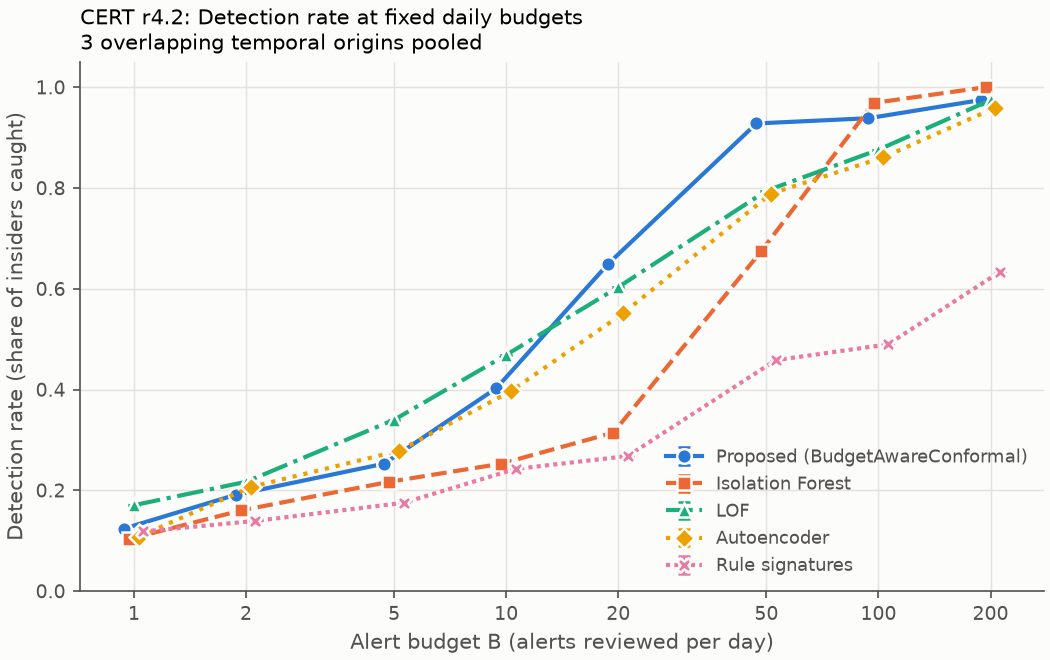
\includegraphics[width=\columnwidth]{figures/dr_vs_budget.png}
\caption{Detection rate against the daily alert budget on the CERT r4.2 test windows (95\% bootstrap
CI over insiders where available).}
\label{fig:budget}
\end{figure}

\subsection{Scenarios}
Table~\ref{tab:scenario} splits the detection rate at 10 alerts per day by scenario.
% Hand-written narrative; numbers are macros.
All detectors except the signature rules find the three S3 administrators who log in as their
supervisor (\DROursSThree{} for ours): new-PC logons, after-hours activity and a burst of e-mail make
those days stand out. About half of the S1 insiders, who copy data to USB after hours and visit a leak
site, are caught by every method (\DROursSOne{} for ours, \DRIFSOne{} for Isolation Forest). S2,
month-long job hunting followed by data theft, is where the methods separate: Isolation Forest
catches \DRIFSTwo{} of these insiders, BudgetAwareConformal \DROursSTwo{} and LOF \DRLOFSTwo. Their
individual days look ordinary to a population model; they stand out only against the user's own
history, and only on a few days of their month-long malicious period.


\begin{table}[t]
\centering
\caption{Detection rate at 10 alerts/day per insider scenario (insiders pooled over origins).}
\label{tab:scenario}
\begin{tabular}{lccc}
\toprule
Detector & S1 (n=13) & S2 (n=17) & S3 (n=3) \\ \midrule
BudgetAwareConformal (ours) & 0.44 & 0.33 & 1.00 \\
Isolation Forest & 0.45 & 0.03 & 1.00 \\
LOF & 0.38 & 0.41 & 1.00 \\
Autoencoder & 0.47 & 0.32 & 1.00 \\
Rule signatures & 0.46 & 0.15 & 0.33 \\

\bottomrule
\end{tabular}
\end{table}

\subsection{Ablation}
% Hand-written narrative; numbers are macros.
Table~\ref{tab:ablation} changes one component at a time on the same test windows (seeds 0--2).
The per-user baseline (C1) carries the method: replacing it with a population baseline drops the
detection rate from \AblFullDR{} to \AblNoCOneDR{} and the precision from \AblFullP{} to
\AblNoCOneP{}, the level of Isolation Forest. Removing the resource family lowers the detection rate
to \AblNoResourceDR{}, and removing the volume family lowers the precision to \AblNoVolumeP{}.
Repeat-alert suppression (C4), switched off by tuning, lowers precision (\AblCFourP).

Several variants do \emph{better} on the test windows than the tuned model: Fisher fusion
(DR \AblFisherDR, P \AblFisherP), no calibration (DR \AblNoCTwoDR, P \AblNoCTwoP) and dropping the
identity family (DR \AblNoIdentityDR, P \AblNoIdentityP). Validation had preferred the tuned
settings (validation DR@10 \ValDROurs{} for the selected configuration). We do not switch to any of
these variants, because choosing among them now would select on the test windows; we report the gap
as evidence that the short development period, whose validation windows hold fewer insiders than
the test windows, is a weak guide to the later months.

\begin{table}[t]
\centering
\caption{Ablation at 10 alerts/day on the test windows (DR with 95\% CI over insiders; P@10).}
\label{tab:ablation}
\resizebox{\columnwidth}{!}{%
\begin{tabular}{lcc}
\toprule
Variant & DR@10 [95\% CI] & P@10 \\
\midrule
Full (tuned) & 0.43 [0.28, 0.60] & 0.028 \\
-C1 population baseline & 0.28 [0.14, 0.44] & 0.007 \\
-C2 no calibration & 0.63 [0.47, 0.79] & 0.021 \\
-C3 no fusion (pooled) & 0.56 [0.39, 0.72] & 0.019 \\
+C4 suppress 3 d & 0.43 [0.27, 0.58] & 0.018 \\
-identity family & 0.55 [0.39, 0.71] & 0.034 \\
-resource family & 0.30 [0.17, 0.45] & 0.029 \\
-temporal family & 0.49 [0.34, 0.66] & 0.028 \\
-volume family & 0.39 [0.24, 0.57] & 0.009 \\
fusion: fisher & 0.61 [0.45, 0.76] & 0.025 \\
fusion: harmonic & 0.49 [0.33, 0.65] & 0.029 \\
fusion: stouffer & 0.17 [0.06, 0.30] & 0.006 \\
Isolation Forest (reference) & 0.29 [0.15, 0.45] & 0.007 \\

\bottomrule
\end{tabular}}
\end{table}


\subsection{Explanations and triage (O3, O4)}
% Hand-written narrative; numbers are macros.
Across all \ExpNAlerts{} alerts the frozen detector emits at 10 alerts per day on the test windows
(\ExpNTrue{} true), the family an explanation names is itself informative (Table~\ref{tab:family}).
Alerts explained by a \emph{volume} deviation are true \ExpVolPrec\% of the time, against
\ExpAllPrec\% over all alerts, and they account for \ExpVolShareTrue\% of the true alerts; no alert
explained by an \emph{identity} deviation was true (\ExpIdnPrec\%), in line with the ablation. An
analyst who works the queue by explanation type rather than by rank would reach true alerts sooner.
% Hand-written narrative; numbers are macros.
As an independent check of faithfulness, Kernel SHAP~\cite{lundberg2017shap} was run on the
detector's score for \ShapN{} alerts of one test window, with each user's usual feature vector as
the baseline. SHAP's top-ranked feature is one of the features the explanation names in
\ShapTopNamed\% of alerts, and it lies in the explanation's primary family in \ShapFamilyAgree\%.


Whether a person can triage from the explanation alone (H3) is tested by a pre-registered crossover
study: \StudyN{} alerts (\StudyTrue{} true, from \StudyInsiders{} insiders across all three
scenarios, and \StudyFalse{} false), two arms
(score only vs.\ explanation only), four reviewers, each alert judged twice per arm by different
people, and a paired bootstrap over alerts on balanced accuracy. The study is \TriageStatus{}
(Table~\ref{tab:triage}); all \TriageNUsable{} of \TriageNExpected{} planned judgements were usable.
Reviewers shown only the explanation reached a balanced accuracy of \TriageBAB{}, against
\TriageBAA{} for reviewers shown only the score, a difference of \TriageDiff{} percentage points
(95\% CI \TriageLo{} to \TriageHi{}). The entire interval lies above the pre-registered
+\TriageThr{} points threshold, so H3 is \textsc{\TriageVerdict}. Reviewers in arm~B were
substantially more accurate on both true alerts (sensitivity \TriageSensB{}) and false alerts
(specificity \TriageSpecB{}), and they expressed higher confidence and spent roughly twice as long
per alert (mean confidence 4.2 vs.\ 2.2 in arm~A), consistent with reading a
richer explanation. In arm~A, near-chance balanced accuracy (\TriageBAA{}) confirms that the bare
anomaly score carries little actionable signal at the presented granularity. Inter-rater agreement
was higher in arm~B than arm~A (Cohen's $\kappa$: \TriageKappas), suggesting the explanation
creates a shared basis for judgment
that the score alone does not. By explanation family, arm-B accuracy was
\TriageFamIdn{} for identity, \TriageFamRes{} for resource, \TriageFamTmp{} for timing and
\TriageFamVol{} for volume explanations; performance was consistent across families, with
identity-deviation alerts reaching perfect accuracy (Table~\ref{tab:family}).

\begin{table}[t]
\centering
\caption{Triage study (H3): judgements pooled over four reviewers, 40 alerts (20 true).}
\label{tab:triage}
\resizebox{\columnwidth}{!}{%
\begin{tabular}{lcccccc}
\toprule
Arm & $n$ & Bal.\ acc. & Sens. & Spec. & Conf. & Sec. \\
\midrule
Score only & 80 & 0.475 & 0.62 & 0.33 & 2.2 & 19 \\
Explanation only & 80 & 0.913 & 0.90 & 0.93 & 4.2 & 40 \\

\bottomrule
\end{tabular}}
\end{table}

\begin{table}[t]
\centering
\caption{Precision of alerts by the behaviour family their explanation names (10 alerts/day, CERT
test windows, \ExpNAlerts{} alerts).}
\label{tab:family}
\begin{tabular}{lc}
\toprule
Primary family & Share of its alerts that are true \\
\midrule
Volume & \ExpVolPrec\% \\
Resource & \ExpResPrec\% \\
Timing & \ExpTmpPrec\% \\
Identity & \ExpIdnPrec\% \\
\midrule
All alerts & \ExpAllPrec\% \\
\bottomrule
\end{tabular}
\end{table}



% ---------------------------------------------------------------------------------------------
\section{Discussion}
% Hand-written narrative; numbers are macros.
\textbf{Choosing the budget.} The budget matters more than the detector. Going from 10 to 50 alerts
per day raises BudgetAwareConformal's detection rate from \DROursBA{} to \DROursBB{} and Isolation
Forest's from \DRIFBA{} to \DRIFBB{}, while precision falls only from \POursBA{} to \POursBB{}
(Fig.~\ref{fig:precision}). Because precision is already far below its ceiling, the extra alerts are
cheap in relative terms; a team that can review 50 alerts a day gains far more from the detector
than one limited to 10.

\textbf{Precision or coverage.} At 10 alerts per day LOF and the autoencoder cover a similar share of
insiders but raise roughly twice as many false alerts per true one. Where analyst time is the
binding constraint, the per-user detector is the better choice; where missing an insider is far
costlier than reviewing false alerts, a density baseline is a reasonable complement, and the two
could share one queue.

\textbf{Working the queue by explanation.} Ranking only by score ignores information the detector
already produces. Since volume-explained alerts are true several times more often than the rest
(Table~\ref{tab:family}), an analyst can triage those first; identity-only deviations (new PCs) were
never malicious in our test windows.

\textbf{Organisation size and cost.} The budget is fixed per day, so the same 10 alerts cover a
larger share of a smaller organisation. On random samples of \NUsersSmall{} and \NUsersMid{} users the
detection rate at 10 alerts per day is \DRSweepOursSmall{} and \DRSweepOursMid{} for our detector
(Isolation Forest \DRSweepIFSmall{} and \DRSweepIFMid), against \DRSweepOursFull{} on all
\NUsersFull{} users (Fig.~\ref{fig:scale}; means over runs, hence slightly different from the
insider-pooled estimate of Table~\ref{tab:main}). Fitting and scoring one test window on all users takes
\SecsOurs\,s for BudgetAwareConformal, against \SecsIF\,s for Isolation Forest, \SecsLOF\,s for LOF
and \SecsAE\,s for the autoencoder.

\begin{figure}[t]
\centering
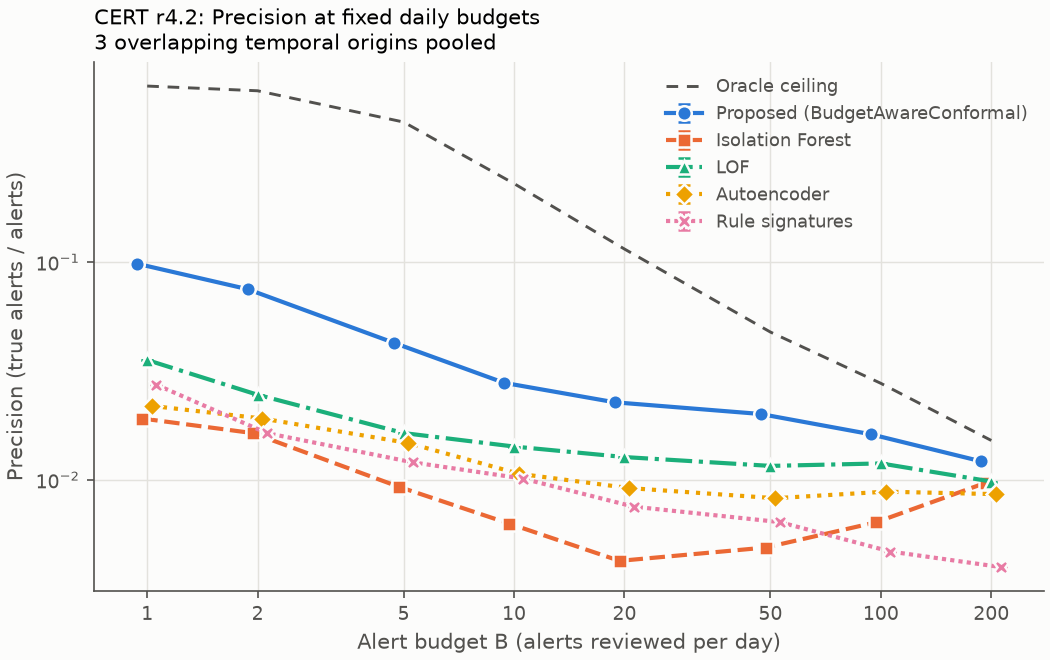
\includegraphics[width=\columnwidth]{figures/precision_vs_budget.png}
\caption{Precision against the daily alert budget (log scales) with the oracle ceiling, CERT r4.2
test windows.}
\label{fig:precision}
\end{figure}

\begin{figure}[t]
\centering
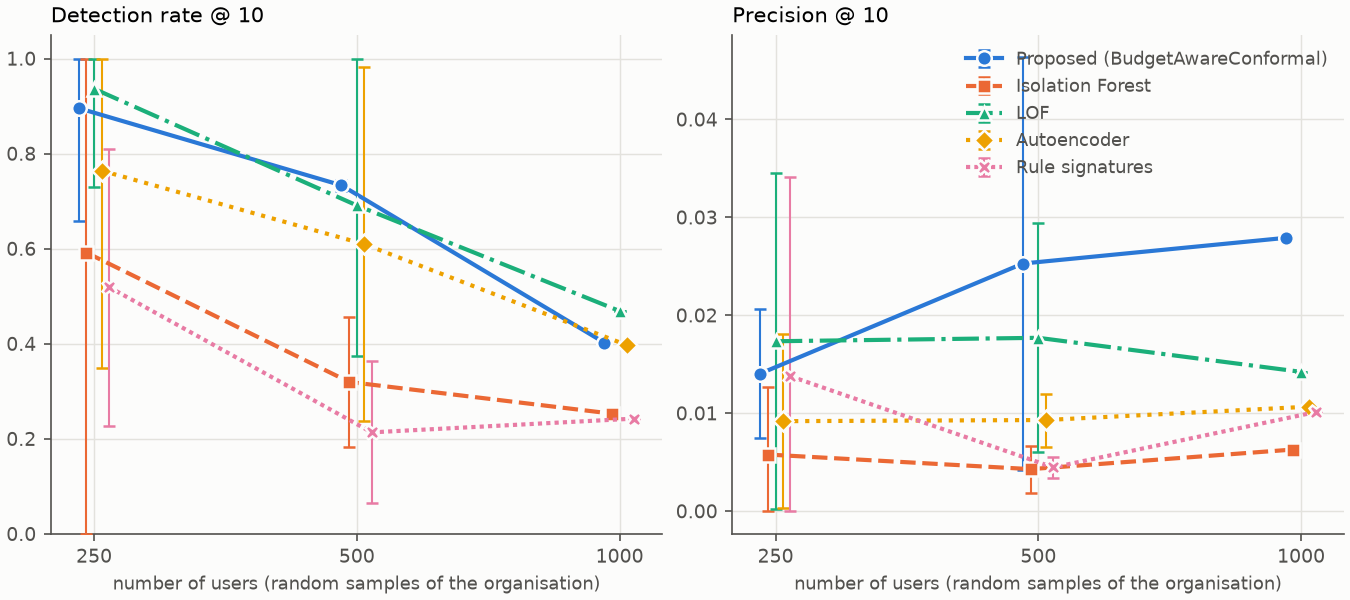
\includegraphics[width=\columnwidth]{figures/sweep_principals.png}
\caption{Detection rate and precision at 10 alerts/day on random samples of the organisation (three
samples per size; 95\% $t$-interval over samples).}
\label{fig:scale}
\end{figure}


% ---------------------------------------------------------------------------------------------
\section{Analyst Console}
A Streamlit console applies the frozen model to uploaded CERT-format logs: it parses the CSVs with
the same code as the benchmark, builds the causal features over the uploaded period (the first two
weeks serve as history), scores every user-day with all five detectors, and shows the daily queue
at a chosen budget with the explanation, family $p$-values and any signature rules that also fired.
Optional labels yield precision and insiders caught; alerts and scores are exported as CSV.

% ---------------------------------------------------------------------------------------------
\section{Limitations and Threats to Validity}
CERT r4.2 is generated by a simulator, contains no cloud logs, and is one organisation; results
are not replicated across independent datasets. Only \NInsTest{} insiders fall in the test windows,
so intervals on the detection rate are wide. Validation detection was markedly higher than test
detection, which points to drift between the development period and the later months. The keyword
lists use the kinds of sites named in the public scenario descriptions. The triage study (H3) is
small (4 reviewers, 40 alerts) and its reviewers are the system's authors, who may know the public CERT scenario
descriptions. Its 50\% share of true alerts is far above the share in the live queue, so its
accuracy is not operational accuracy; balanced accuracy is reported for that reason.

\section{Conclusion}
% Hand-written narrative; numbers are macros.
Evaluated where a SOC actually operates, at a fixed number of alerts per day, judging each user
against their own history with pooled conformal calibration roughly quadruples the precision of
Isolation Forest on CERT r4.2 (\POursBA{} vs.\ \PIFBA{} at 10 alerts per day) and gives the highest
precision of all five detectors at every budget, while fitting in under a second. It does not
reliably detect more insiders at 10 alerts per day than Isolation Forest, LOF or an autoencoder
(H1a and H2 not supported), although at 50 alerts per day it reaches \DROursBB{} against \DRIFBB{}.
The ablation locates the gain in the per-user baseline and shows that the settings chosen on a
short development period did not transfer fully to later months. Every alert names the behaviour
that deviated, and in our pre-registered triage study reviewers shown only the explanation triaged
alerts with a balanced accuracy of \TriageBAB{} against \TriageBAA{} for the score-only arm
(\TriageDiff{} points, 95\% CI \TriageLo{} to \TriageHi{}; H3 \TriageVerdict{}), confirming that
the explanations carry actionable signal. Future work: a longer development period or rolling
re-tuning, the remaining CERT releases and real cloud control-plane logs, and replication of the
triage finding with independent analysts on a larger alert set.


\bibliographystyle{IEEEtran}
\bibliography{references}

\end{document}
